\begin{frame}{Quantum particles in a quasiperiodic (QP) environment}
\begin{columns}
\begin{column}{0.5\textwidth}
QP environment: Fibonacci chain
\centering
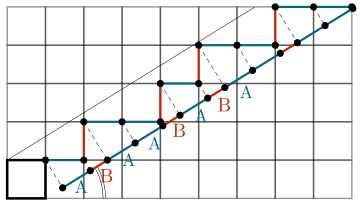
\includegraphics[width=0.8\textwidth]{img/3_Fibonacci/full_cp}
\end{column}
%%%%%%%%%%%%%
\begin{column}{0.5\textwidth}
Quantum particles: fermions
\centering
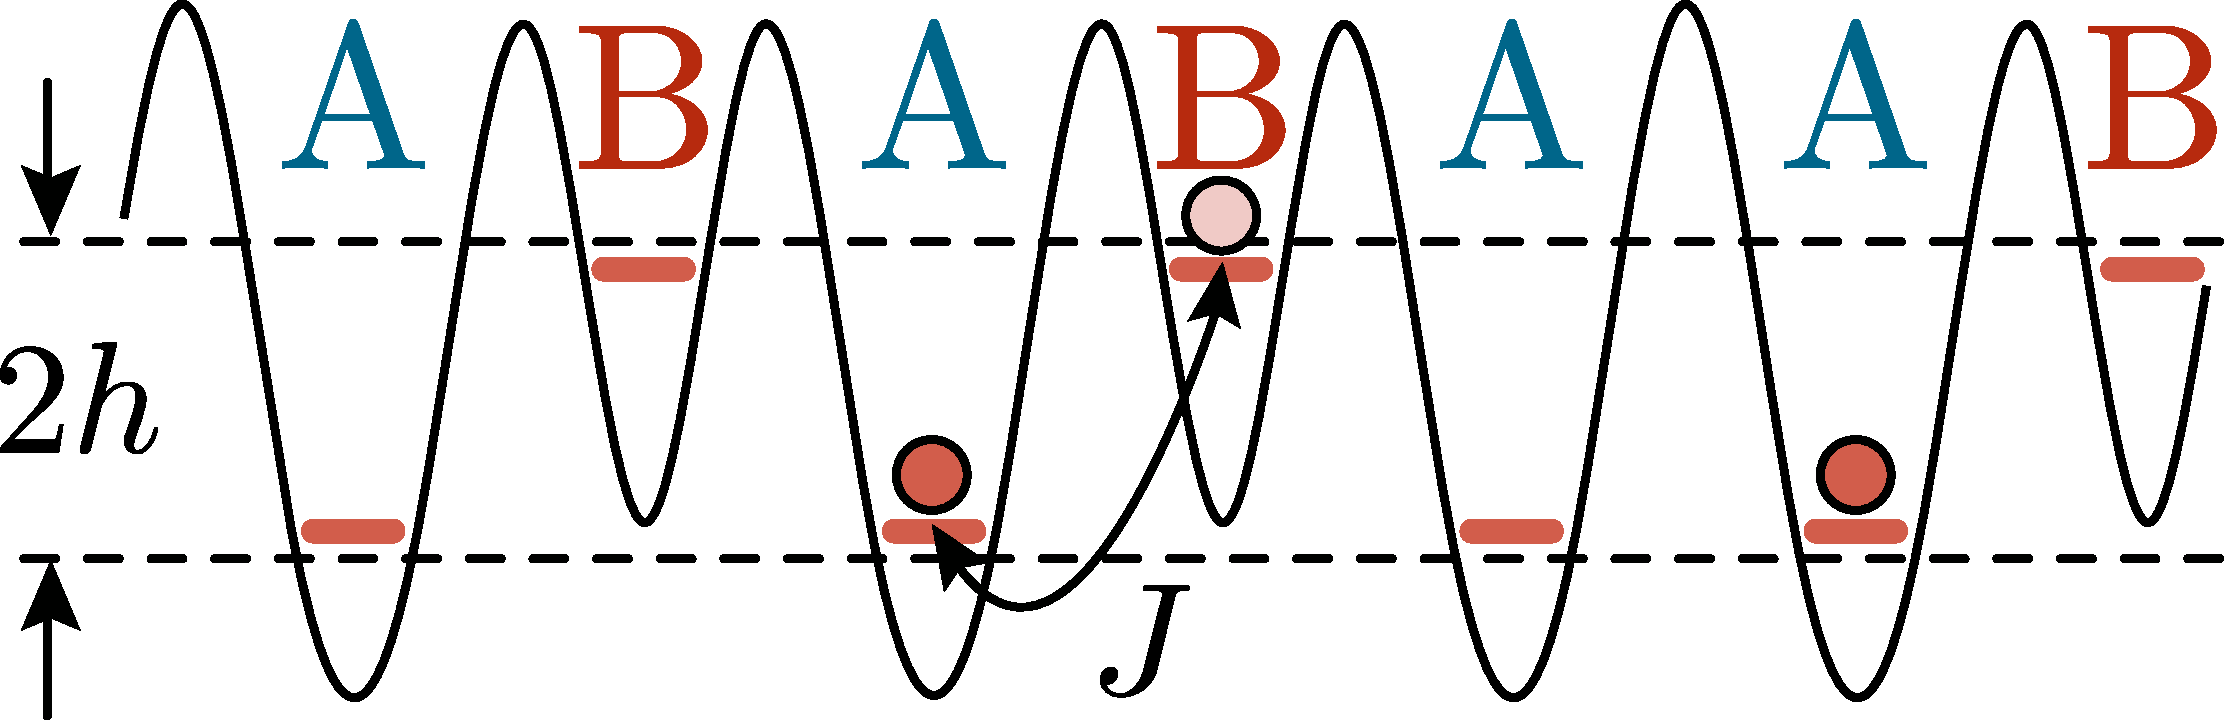
\includegraphics[width=0.7\textwidth]{img/1_motivation/XXZ_QP_cold_atoms}
\[
	H = \sum_{i=1}^L \left[ J (c_i^\dagger c_{i+1} + \text{h.c}) - h_i n_i \right]
\]
\end{column}
\end{columns}
\centering
\textbf{Multifractal} (scale invariant) states

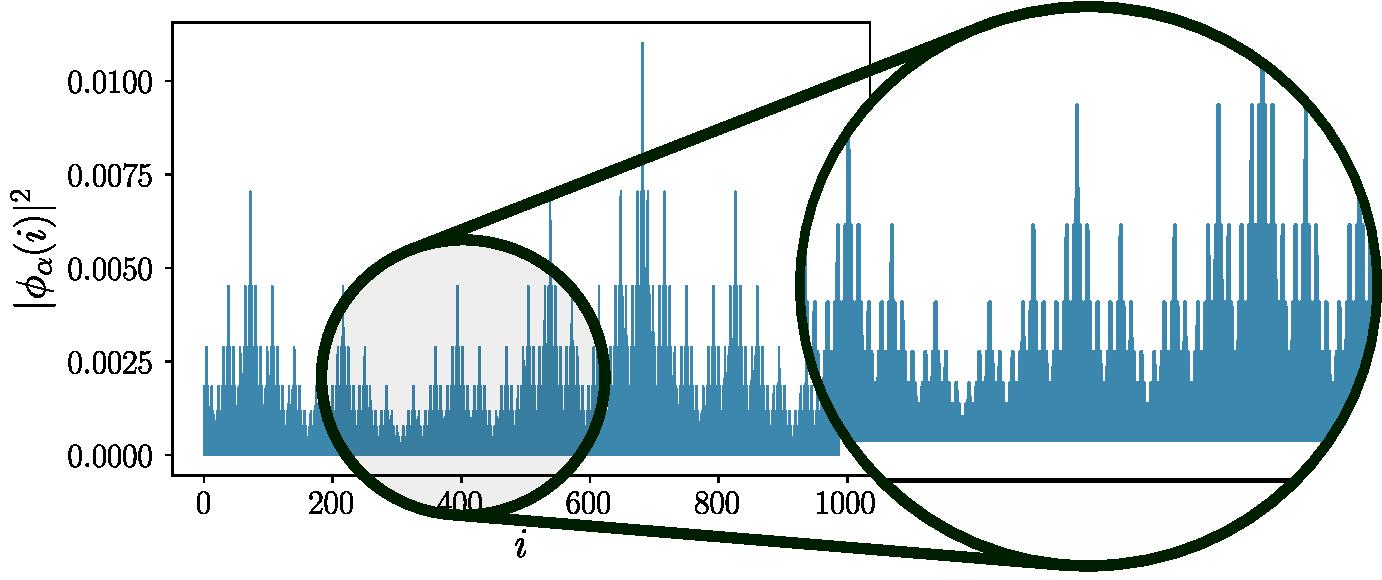
\includegraphics[width=0.4\textwidth]{img/1_motivation/one_density_zoom}
\end{frame}

\begin{frame}{Motivation: quasiperiodicity + interacting electrons}
\textbf{No interactions}:

{
\centering
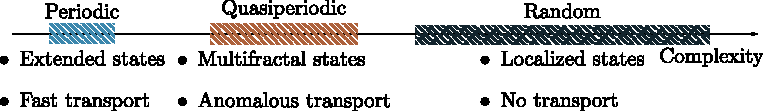
\includegraphics[width=\textwidth]{img/1_motivation/complexity.pdf}

}

Quasiperiodicity (QP) + \textbf{interactions} between particles?

\begin{columns}
\begin{column}{0.4\textwidth}
\centering
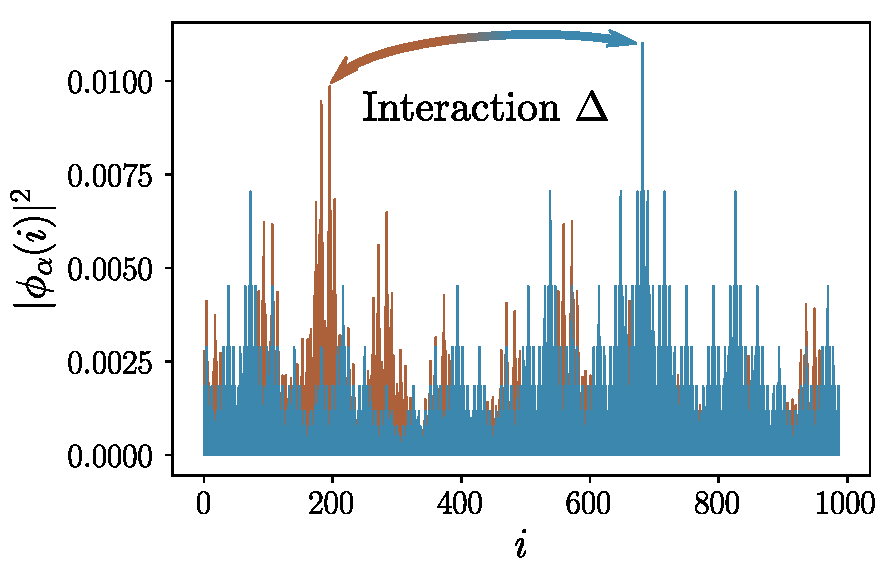
\includegraphics[height=3.5cm]{img/0_cover/free_two_densities_interaction}
\end{column}
\begin{column}{0.6\textwidth}

Naively: delocalisation, fast transport

\textbf{Results}: 
\begin{itemize}
	\item weak QP: delocalisation, fast transport
	\item strong QP: \textbf{many-body localisation}, no transport
\end{itemize}
\end{column}
\end{columns}
\end{frame}